\chapter{Asking San Francisco Millionaires How They Got Rich!}

This chapter follows a School of Hard Knocks street interview, curated by LazyingArt LLC, in which San Francisco is treated not as scenery but as a working environment for studying wealth. The lecture is valuable because it does not offer one unified theory of riches. Instead, it unfolds a sequence of money grammars in time: conservative retention, founder conviction, venture asymmetry, priced political uncertainty, and finally the slower, harsher logic of principal-to-principal real estate. We preserve that order, because the lecture itself makes its points by moving through the city and discovering what each stop can support.

\section{Cold Open and San Francisco as a Wealth Field}

The lecture opens by spending outcomes before causes. We hear, in quick succession, that somebody in venture capital made roughly fifty million dollars in a year, that a company moved from a five-million-dollar valuation to roughly 2.1 billion, that a Ferrari owner is in commercial real estate, and that age-at-millionaire questions will matter. The function of this cold open is not explanation. It is promise. The lecture tells us at once that the city contains numbers large enough to be worth interrogating.

Only after that teaser does the host widen the frame. San Francisco is introduced as a dense wealth field. The city's scale is given explicitly:
\begin{equation}
N_{\text{millionaires}} > 300{,}000,\qquad
N_{\text{billionaires}} > 80.
\end{equation}
The host also calls San Francisco the second wealthiest city in the world and claims that billionaire concentration here is exceptionally high. We keep these as host-attributed setup claims. Their role is motivational: they justify why this city, and not some ordinary street, is where the inquiry will be run.

One of the lecture's most important numerical motifs also appears here. A large valuation path is announced before we know whose path it is:
\begin{equation}
V_{\text{startup}}:\ \$5\,\text{million}\to \$2.1\,\text{billion}.
\end{equation}
If we simply normalize the two endpoint figures, the scale jump becomes
\begin{align}
V_0 &= \$5\,\text{million}, &
V_1 &= \$2.1\,\text{billion},\\
\frac{V_1}{V_0} &= \frac{2.1\,\text{billion}}{5\,\text{million}} = 420.
\end{align}
The lecture does not say ``420x,'' but the arithmetic is useful because it shows exactly what sort of magnitude the teaser is promising. As usual in this series, scale is introduced first and defined only later.

\section{Marina District: Refusal, Search, and the First Money Rule}

The next move is essential to the lecture's rhythm. Instead of dropping immediately into rich doctrine, the host takes us into the Marina District and lets us feel how difficult it is to get access at all. We are near ``Billionaires' Row,'' but the first thing the city yields is not wisdom. It is resistance.

Several attempts fail. One passerby refuses the game. Another asks who the cameraman is and does not want to appear on camera. Another says he has to fix his phone. The lecture then pauses and interprets its own failure. This matters. A weaker chapter would cut these moments as dead air. But the lecture wants the refusals to become part of the teaching. Wealth is not only a distribution of assets. It is also a distribution of social access.

The first stable doctrine comes from an older finance speaker who says he became a millionaire in his late thirties and is now seventy. He worked in the stock market, was on Wall Street, and once made eight figures in a single year. Yet the important point is not the annual number. It is the distinction he draws between making money and keeping it. His advice is to work hard, invest conservatively, and remember that many people make a great deal of money without retaining much of it.

That distinction is elementary, but the lecture places it here for a reason. We begin with a city of huge outcomes, and the first mature voice warns us that flow and stock are not identical. A large income in one year is not the same thing as durable capital over time.

The host then turns the failed interviews into a rule: every no is one step closer to a yes. In note form, the point is not that refusals are good in themselves. It is that refusals do not terminate the search:
\begin{equation}
N_{\text{no}}\uparrow \;\not\Rightarrow\; \text{search ends}.
\end{equation}

\subsection{Question \& Answer}

\paragraph{Question.} Why does access friction belong in a lecture about wealth?

\paragraph{Answer.} Because in this lecture access friction is part of the mechanism of discovery. The host is not teaching from a studio. He is extracting doctrine from a city whose wealthy people are hurried, suspicious of cameras, and often unwilling to stop. The repeated refusals therefore do not merely delay the lecture; they explain the lecture. Commercial knowledge is socially gated, and persistence is one of the conditions under which that gate is opened.

\section{The AI Founder: Conviction, Product-Market Fit, and Payroll}

Only after the access-friction beat does the lecture land its first full founder case. The speaker says he is in tech, owns a company, has been a business owner for about ten years, and names the firm as Cantina. It is an artificial-intelligence business, and he says this is roughly his seventh company. In scale terms, he reports a year at about fifty million dollars in revenue:
\begin{equation}
N_{\text{companies}} \approx 7,\qquad
T_{\text{owner}} \approx 10\ \text{years},\qquad
R_{\max} \approx \$50\,\text{million/year}.
\end{equation}

The lecture then shifts from endpoint to mechanism. He says he never went to college because he never wanted to go and never found value in it. That point by itself is not the thesis. The real thesis comes next. One must find something one actually loves to do, do it repeatedly, and keep doing it until one finds product-market fit. The lecture does not formalize that condition, but the operational direction is clear:
\begin{equation}
\text{repeat the work} \;\Rightarrow\; \text{eventual product-market fit}.
\end{equation}
We should read the arrow cautiously. It is heuristic, not deterministic. The point is not that repetition guarantees fit. It is that repetition is meaningful only when anchored in conviction.

The speaker then sharpens the idea. One cannot do this merely for money. One must have a real idea, and one must care about it enough to keep pressing after loss. The lecture immediately tests that claim by asking about loss. The answer is: lots. What gives the section its real force is the payroll story. The low point is not a vague period of stress. It is the moment when one must pull money out of one's own checking account to make payroll so that employees do not have to be let go.

This is where the lecture's rhetoric about entrepreneurship earns its right to exist. When the founder says that not everybody is built for entrepreneurship, the claim is anchored by a concrete mechanism: personal absorption of liquidity pressure. Without that story, the line would be motivational fluff. With it, it becomes an operating distinction.

The section ends with negotiation. The founder says not to get too wrapped up in outcome. When the host translates that into a sales question, the founder tightens it further: the best way to sell something is not to sell it. That is not a denial of persuasion. It is a warning against obvious need.

\subsection{Question \& Answer}

\paragraph{Question.} Why does caring too much about the outcome weaken selling and negotiation?

\paragraph{Answer.} Because visible need changes posture. If we require one deal too badly, we reveal pressure, and that pressure can be read by the other side. The lecture's point is therefore structural rather than psychological:
\begin{equation}
\text{attachment to outcome}\uparrow \;\Rightarrow\; \text{selling quality}\downarrow.
\end{equation}
The founder's advice here will later rhyme with the real-estate advice: in both domains, desperation leaks information.

\section{Election Markets and State-Level Narrowing}

At this point the lecture interrupts itself. Before moving to the next interview, the host pivots into a sponsor segment about election betting. The interruption should be preserved as an interruption. It does not belong to the core entrepreneurial doctrine, but it does briefly change the lecture's form. Instead of interviewing a person, the host interviews a market.

The sponsor claims are given directly in probability and volume language:
\begin{equation}
p_{\text{Trump}} \approx 0.60,\qquad
p_{\text{Kamala}} \approx 0.40,
\end{equation}
and
\begin{equation}
V_{\text{platform}} > \$1\,\text{billion},\qquad
D=\$100 \Rightarrow C=\$20.
\end{equation}
The lecture then narrows from the general election to swing states. This narrowing is important because it shifts the level of analysis from a national headline to state-by-state resolution.

Arizona is shown not as a visible odds table, but as a locator graphic. The safest notation we may place beside that figure is minimal:
\begin{equation}
s=\text{Arizona},\qquad
p_s=\Pr(\text{candidate wins state } s).
\end{equation}
The second symbol is a note-writer's abstraction only. It is not shown in the frame.

\begin{figure}[h]
\centering

\includegraphics[width=0.82\textwidth]{lecture_62_figure_02.png}
\caption{Arizona swing-state locator graphic. The lecture is narrowing to a state-level market example, not displaying a visible state probability.}
\end{figure}

To keep the visual interpretation honest, we can pair the screenshot with a stripped-down schematic. The point is not to redraw a forecast map. It is only to record the lecture's state-level narrowing.
\begin{figure}[h]
\centering
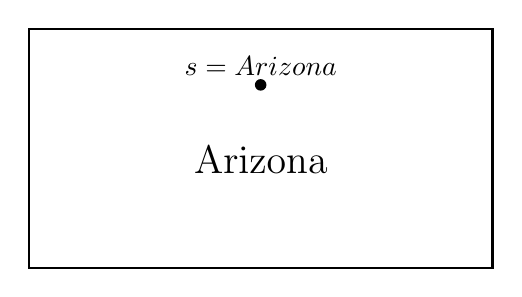
\begin{tikzpicture}[scale=0.95]
\draw[thick] (0,0) rectangle (6.2,3.2);
\node at (3.1,1.45) {\Large Arizona};
\fill (3.1,2.45) circle (2.2pt);
\node[above] at (3.1,2.45) {$s=\text{Arizona}$};
\end{tikzpicture}
\caption{Minimal reconstruction of the lecture's state-level focus. We retain only the singled-out state \(s\), not any unshown probability or margin.}
\end{figure}

The visual evidence is useful precisely because it is modest. Arizona is isolated, labeled, and pinned. We are shown the level at which the market may be narrowed. We are not shown a state probability, a vote share, or a map legend.

\section{Venture Capital as Portfolio Arithmetic}

After the sponsor interruption, the lecture returns to commercial doctrine in a more arithmetical mode. A venture-capital speaker says he became a millionaire at about twenty-eight and is now fifty-eight. When asked how venture capital makes money, he gives the cleanest distributional rule in the lecture: invest in thirty companies, expect twenty-five to go to zero, and rely on five that may pay off one hundred-fold or two hundred-fold.

This is the lecture's clearest asymmetry model:
\begin{equation}
N_{\text{portfolio}}=30,\qquad
N_{0}=25,\qquad
N_{+}=5,
\end{equation}
with the surviving-return scale
\begin{equation}
m_{+}\approx 100\times \text{ to } 200\times.
\end{equation}
The portfolio shares make the structure visible:
\begin{align}
\frac{N_0}{N_{\text{portfolio}}} &= \frac{25}{30}=\frac{5}{6},\\
\frac{N_+}{N_{\text{portfolio}}} &= \frac{5}{30}=\frac{1}{6}.
\end{align}
So roughly five sixths of the positions can fail outright, while roughly one sixth carries the upside.

To see the arithmetic more concretely, let us normalize each investment to one unit of capital. If twenty-five positions go to zero and five return \(100\times\), then the gross return units are
\begin{equation}
25\cdot 0 + 5\cdot 100 = 500,
\end{equation}
so the gross portfolio multiple on the original thirty units is
\begin{equation}
\frac{500}{30}\approx 16.7\times.
\end{equation}
If instead the five winners return \(200\times\), then
\begin{equation}
\frac{25\cdot 0 + 5\cdot 200}{30}=\frac{1000}{30}\approx 33.3\times.
\end{equation}
This is not the speaker's explicit calculation, but it is the natural worked example implied by his rule. It shows why a portfolio with many zeros can still be extraordinarily successful.

The same speaker then grounds the arithmetic in biography. He says he became a millionaire by saving money, getting good jobs, moving around, and hustling. The host paraphrases: the more hands we shake, the more money we make. The speaker even says, then softens, that most people cannot become millionaires working from home. The real point is not the prohibition. It is that contact density, movement, and professional exposure are treated as money-making variables.

The best investment, he says, was a company he started himself, RxList. He put in his own money, raised no venture capital, grew it for about three and a half years, and sold it to WebMD at roughly a \(33\times\) result:
\begin{equation}
M_{\text{RxList}} \approx 33\times,\qquad
T_{\text{RxList}} \approx 3.5\ \text{years}.
\end{equation}
This matters because it lets the lecture distinguish between investor arithmetic and operator ownership. The same person is describing both, but the mechanism is different in each case.

The later valuation story returns as well. A company called ``Metable'' in the transcript is said to have moved from a five-million-dollar first-round valuation to roughly 2.1 billion most recently. The speaker says that does not yet make him a billionaire. The lecture is therefore careful, whether deliberately or incidentally, about not confusing company valuation with personal net worth.

The section closes with scaling doctrine. The most common mistake in business, according to this speaker, is failure to hire A players, put good people around oneself, and delegate. One must be willing to give other people responsibility, even responsibility they may perform better than one performs it oneself. Then comes the soft but important close: get along with people, be a sponge, absorb information, and do not let fear of mistakes freeze action.

\subsection{Question \& Answer}

\paragraph{Question.} How can a portfolio survive when most companies go to zero?

\paragraph{Answer.} Because the lecture is describing a regime in which a small number of outcomes dominate the total. In ordinary language, we do not need the typical company to work. We need a few companies to work disproportionately well. The arithmetic above makes the point explicit. Many zeros do not destroy the portfolio if the rare winners are sufficiently large.

\section{Financial District and the Real-Estate Operator}

The lecture now changes geography once again. We move to the financial district, called the Wall Street of the West Coast, and the access-friction motif returns in harsher form. Finance people are in meetings, moving between buildings, and are even harder to stop than people in the Marina. The transcript becomes partially garbled in this stretch, so we keep only the coherent doctrine that survives later in the segment.

A later commercial-real-estate operator says he owns about 100,000 square feet, makes about half a million dollars personally in a year, and that the business does about one million:
\begin{equation}
A_{\text{owned}} \approx 100{,}000\ \text{sq ft},\qquad
Y_{\text{personal}} \approx \$500{,}000,\qquad
R_{\text{business}} \approx \$1\,\text{million}.
\end{equation}
He says he became a millionaire at about thirty-eight and is now sixty:
\begin{equation}
a_{\text{millionaire}}=38,\qquad
a_{\text{now}}=60.
\end{equation}

His negotiation advice is cleaner than it first sounds. Negotiate with the other principal. Do not let anybody get in the middle of the deal. Brokers may be good people, but once they dominate the exchange, direct control of terms weakens:
\begin{equation}
\text{middleman in the deal} \;\Rightarrow\; \text{direct control of terms}\downarrow.
\end{equation}
This sits naturally beside the founder's earlier warning about caring too much about one outcome. In both cases, we are being told to reduce sources of weakness.

The timing rule for real estate is equally direct. Buy when people are selling. The explanation is not mystical. Seller urgency increases supply and depresses price:
\begin{equation}
S_{\text{sellers}}\uparrow \;\Rightarrow\; P_{\text{asset}}\downarrow.
\end{equation}
This is not a full market-clearing derivation. It is a directional heuristic, and the lecture wants it exactly in that form.

The same operator speaks in a strongly pro-leverage register, saying in effect that debt is how real estate is bought. Here we remain cautious. The lecture gives us a practitioner's rhetoric, not a universal theorem. But the logic is still clear: leverage is presented as the mechanism by which asset control scales beyond immediate cash.

The final texture of the section is personal rather than algebraic. The operator recalls downturns, says one must keep one's head down and keep plowing through them, and then links money to faith, health, and sacrifice. This is not a detachable moral appendix. It is the lecture's closing reminder that long-horizon asset accumulation depends on staying alive, disciplined, and solvent long enough to exploit timing.

\subsection{Question \& Answer}

\paragraph{Question.} What is the real buying signal in a real-estate downturn?

\paragraph{Answer.} The lecture's answer is not simply ``lower prices.'' It is seller pressure. We are told to buy when people need to get out. In that condition, supply thickens, bargaining power shifts, and terms improve. The signal is therefore not price in isolation, but price under pressure.

\section{Summary}

The lecture begins with endpoints and only later earns the right to explain them. That is its governing rhythm. We move from teaser wealth, to San Francisco as a concentrated wealth field, to the social difficulty of gaining access, to the first conservative rule about keeping money, to a founder's rule about conviction and payroll pain, to an interruption in which politics becomes market probability, to venture capital as a book of many zeros and a few outsized wins, and finally to real estate as timing, principal-to-principal negotiation, leverage, and endurance.

The deepest through-line is that wealth here is not one object. It is search friction, retention, iteration, asymmetry, delegation, and timing. The lecture never collapses those into a single formula, and the chapter should not try to do so. Its strength lies precisely in letting the city unfold one money grammar at a time.